\chapter{Pembuatan Halaman Web Berbasis ABS}

Bab ini memaparkan secara kronologis tentang proses eksperimen yang telah dilakukan oleh penulis untuk mencoba menghasilkan sebuah halaman web dengan menggunakan bahasa pemodelan ABS.

\section{Proses Integrasi ABS dengan JAVA}
Berdasarkan hasil studi literatur yang telah dilakukan, penulis mengetahui bahwa salah satu fitur yang dimiliki oleh ABS adalah kemampuannya untuk dapat di\textit{compile} kedalam bahasa JAVA sehingga nantinya kode ABS tersebut dapat dijalankan di dalam JAVA Runtime Environment (JRE). Berdasarkan informasi tersebut, penulis menarik kesimpulan bahwa jika penulis membuat sebuah JAVA class yang dibuat secara \textit{native}, maka JAVA Class tersebut akan dapat memanggil class ABS yang sudah di\textit{compile} menjadi JAVA Class juga.\\

Sebelum penulis mencoba untuk mengintegrasikan secara langsung ABS dengan JAVA, penulis mencoba untuk mengetahui hasil kompilasi kode ABS yang diubah kedalam JAVA. berikut adalah kode ABS sederhana yang penulis buat beserta hasil kompilasinya ke dalam kode JAVA.

\begin{lstlisting}[
caption=Kode ABS beserta Main Blocknya,
label={lst:absSederhana},
escapeinside={@}{@}
]
module UserModule;

interface User
{
	String getUsername();
}

class UserImpl implements User
{
	String getUsername() @\label{lst:absString}@
	{
		return "salman"; @\label{lst:absString2}@
	}
}

//ABS Main block
{
	User myUser = new local UserImpl(); @\label{lst:absCreateObject}@
	String username = myUser.getUsername(); @\label{lst:absCallMethod}@
}
\end{lstlisting}

Kode \ref{lst:absSederhana} di atas merupakan kode ABS sederhana yang penulis buat untuk mengetahui hasil konversi kode ABS menjadi kode JAVA dalam hal pembuatan objek baru (baris \ref{lst:absCreateObject}), pemanggilan \textit{method} (baris \ref{lst:absCallMethod}) dan konversi data ABS kedalam kode JAVA (baris \ref{lst:absString2}). Kode ini dibuat sebagai langkah awal penulis dalam mempelajari hasil konversi kode ABS kedalam JAVA untuk keperluan integrasi kedua bahasa tersebut.

\begin{lstlisting}[ 
firstnumber=64,
caption=Hasil kompilasi ABS ke JAVA untuk method getUsername(),
label={lst:absjavaGetUsername},
escapeinside={@}{@},
]
// User.abs:10:2: 
public final abs.backend.java.lib.types.ABSString getUsername() {
    ...
    return abs.backend.java.lib.types.ABSString.fromString("salman"); @\label{lst:absjavaString}@
}
\end{lstlisting}

Kode \ref{lst:absjavaGetUsername} diatas merupakan hasil konversi kode ABS ke dalam JAVA untuk kode \ref{lst:absSederhana} baris \ref{lst:absString2} yang telah dibuat sebelumnya. Seperti yang terlihat pada kode tersebut, tipe data \texttt{String} yang digunakan oleh ABS bukanlah tipe data \texttt{String} standar JAVA API melainkan menggunakan \texttt{ABSString}. Berdasarkan kode JAVA di atas, dapat disimpulkan bahwa terdapat perbedaan tipe data yang digunakna oleh ABS dengan standar JAVA API.

\begin{lstlisting}[
caption=Hasil kompilasi ABS ke JAVA untuk Main Block,
label={lst:absjavaMainBlock},
escapeinside={@}{@}
]
package UserModule;
public class Main extends abs.backend.java.lib.runtime.ABSObject {
    public static void main(java.lang.String[] args) throws Exception {
        abs.backend.java.lib.runtime.StartUp.startup(args,Main.class);
    }
    public java.lang.String getClassName() { return "Main"; }
    public java.util.List<java.lang.String> getFieldNames() { return java.util.Collections.EMPTY_LIST; }
    public Main(abs.backend.java.lib.runtime.COG cog) { super(cog); }
    public abs.backend.java.lib.types.ABSUnit run() {
         {
            ...
            UserModule.User_i myUser = UserModule.UserImpl_c.__ABS_createNewObject(this); @\label{lst:absjavaCreateObject}@
            
            ...
            abs.backend.java.lib.types.ABSString username = abs.backend.java.lib.runtime.ABSRuntime.checkForNull(myUser).getUsername();
            if (__ABS_getRuntime().debuggingEnabled()) __ABS_getRuntime().getCurrentTask().setLocalVariable("username",username);
        }
        
        return abs.backend.java.lib.types.ABSUnit.UNIT;
    }
}
\end{lstlisting}

Seperti yang terlihat pada kode \ref{lst:absjavaMainBlock} baris \ref{lst:absjavaCreateObject}, terdapat perbedaan pada kode JAVA hasil kompilasi dari ABS dalam membuat \textit{instance} dari sebuah objek. Dalam bahasa JAVA yang standar, untuk dapat membuat \textit{instance} dari sebuah class adalah dengan menggunakan kata kunci \texttt{new} seperti misalnya \texttt{new UserImpl()}. Sedangkan pada kode JAVA hasil kompilasi ABS menggunakan kata kunci \texttt{\_\_ABS\_createNewObject(this)} yang diakses secara \textit{static}.\\

Berdasarkan hasil percobaan tersebut penulis mengetahui bahwa sintaks ABS yang terdapat pada kode \ref{lst:absSederhana} baris \ref{lst:absCreateObject} adalah \textit{equivalent} dengan sintaks JAVA yang terdapat pada kode \ref{lst:absjavaMainBlock} baris \ref{lst:absjavaCreateObject}. Dengan demikian, penulis dapat menyimpulkan bahwa ketika penulis ingin mencoba untuk memanggil class JAVA hasil kompilasi ABS dari class JAVA yang \textit{native} maka penulis harus melakukan pemanggilan fungsi seperti yang terlihat pada kode kode \ref{lst:absjavaMainBlock} baris \ref{lst:absjavaCreateObject} tersebut.\\

%Selain terdapat perbedaan dalam cara membuat \textit{instance} dari sebuah class, terdapat pula perbedaan pada tipe data yang digunakan oleh JAVA hasil kompilasi dari ABS dengan JAVA yang \textit{native}. Jika kita melihat kode \ref{lst:absSederhana} baris \ref{lst:absString} dan \ref{lst:absString2} penulis menggunakan sebuah tipe data \texttt{String} seperti layaknya tipe data \texttt{String} pada JAVA. Akan tetapi ketika kode ABS tersebut di\textit{compile} kedalam bahasa JAVA, ternyata tipe data \texttt{String} tersebut diubah menjadi \texttt{ABSString} seperti yang terlihat pada kode \ref{lst:absjavaGetUsername} baris \ref{lst:absjavaString}. Berdasarkan hasil percobaan tersebut penulis berkesimpulan bahwa ketika penulis ingin mengintegrasikan ABS dengan JAVA, penulis perlu melakukan konversi tipe data dari tipe data milik JAVA ABS menjadi tipe data standar JAVA.\\

Kesimpulan yang penulis dapatkan setelah melakukan percobaan ini adalah: (1) bahwa untuk dapat membuat sebuah \textit{instance} dari class JAVA hasil kompilasi ABS tidak dapat dilakukan dengan menggunakan kata kunci \texttt{new} seperti pada JAVA yang \textit{native} dan (2) terdapat perbedaan tipe data antara \textit{native} JAVA dengan JAVA hasil kompilasi ABS sehingga perlu adanya penyesuaian lebih lanjut agar penulis dapat mengintegrasikan ABS dengan \textit{native} JAVA.

\section{Pembuatan Halaman Web Sederhana Menggunakan ABS}
Setelah penulis melakukan percobaan sederhana untuk mengetahui cara mengintegrasikan ABS dengan JAVA, selanjutnya penulis melakukan percobaan untuk dapat membuat halaman web sederhana dengan menggunakan ABS. Seperti yang telah kita ketahui bersama, untuk dapat menampilkan sebuah halaman web pada web browser, dibutuhkan adanya sebuah web server yang nantinya akan dapat melayani permintaan dari web browser. Dalam percobaan ini penulis membuat sebuah web server sederhana dengan menggunakan \texttt{ServerSocket} pada JAVA untuk membuka \textit{port} dan menerima \textit{request} dari \textit{web browser} yang nantinya akan memanggil class JAVA hasil kompilasi ABS untuk mendapatkan halaman web yang diinginkan (lihat gambar \ref{fig:howAbsGenerateHTML}).

\begin{figure}
    \centering
    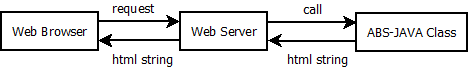
\includegraphics[
        width=0.8\textwidth
    ]{img/request-webserver-abs.png}
    \caption{Bagaimana web server menghasilkan sebuah halaman web}
    \label{fig:howAbsGenerateHTML}
\end{figure}

Untuk dapat mensimulasikan proses seperti yang telah digambarkan pada gambar \ref{fig:howAbsGenerateHTML} di atas, pertama-tama penulis membuat sebuah ABS Module yang fungsinya adalah untuk dapat menghasilkan sebuah halaman sederhana dan memberikannya kepada \textit{web server}. berikut adalah kode ABS yang penulis buat untuk menghasilkan sebuah halaman web:

\begin{lstlisting}[
caption=Kode ABS untuk menghasilkan halaman HTML,
label={lst:absWelcomeView},
]
module ABS.MVC.View.WelcomeView;

interface WelcomeView
{
	String generateView();
}

class WelcomeViewImpl implements WelcomeView
{
	
	String generateView() {		
		String html = "<!DOCTYPE HTML>";
		html = html + "<html>";
		html = html + "<body>";
		html = html + "<h1>Welcome!!</h1>";
		html = html + "Please login <a href='/login.abs'>here</a>";
		html = html + "<br />";
		html = html + "<p>This page was generated from ABS Class</p>";
		html = html + "</body>";
		html = html + "</html>";
		
		return html;
	}
}
\end{lstlisting}

Seperti yang terlihat pada kode \ref{lst:absWelcomeView} di atas, penulis menggunakan \texttt{String} berisikan kode HTML yang disambung-sambung (\textit{concatted String}) untuk menghasilkan sebuah halaman web. Rencananya adalah string yang sudah dihasilkan oleh halaman ABS Module ini nantinya akan diberikan ke \textit{web server} untuk kemudian diberikan ke \textit{web browser} dan ditampilkan ke \textit{user}. Sebagai awalan, penulis membuat sebuah class JAVA yang ditujukan untuk memanggil class JAVA hasil kompilasi ABS tersbut untuk kemudian ditampilkan di \textit{console} dengan menggunakan \texttt{System.out.println()}. Berikut adalah kode JAVA yang dibuat oleh penulis beserta hasil pemanggilan class ABS-nya.

\begin{lstlisting}[
caption=Kode JAVA untuk memanggil ABS,
label={lst:javaCallABS},
escapeinside={@}{@}
]
package com.fmse.absserver;

public class ABSMain extends ABSObject 
{
    ...
       
    public ABSUnit run() {
        System.out.println("ABSMain running..");
        WelcomeView_i view = WelcomeViewImpl_c.__ABS_createNewObject(this); @\label{lst:javaCreateABSObject}@
        ABSString html = ABSRuntime.checkForNull(view).generateView(); @\label{lst:javaCallABSMethod}@
        System.out.println(html.getString());
        return ABSUnit.UNIT; 
    }
    
    public static void main(String[] args) throws Exception {
        StartUp.startup(new String[0], ABSMain.class);
    }
}
\end{lstlisting}

\begin{figure}
    \centering
    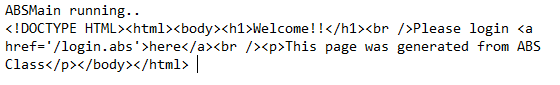
\includegraphics[
        width=0.8\textwidth
    ]{img/java-call-abs-result.png}
    \caption{Hasil dari pemanggilan ABS yang berisikan HTML String}
    \label{fig:javaABSCallResult}
\end{figure}

Terlihat pada kode \ref{lst:javaCallABS} baris \ref{lst:javaCreateABSObject} dan \ref{lst:javaCallABSMethod} di atas, penulis membuat sebuah \textit{instance} dari class \texttt{WelcomView} serta melakukan pemanggilan fungsi \texttt{generateView()} untuk mendapatkan \texttt{String} HTML yang telah dibuat. Hasil dari pemanggilan fungsi \texttt{generateView()} pada class \texttt{WelcomeView} tersebut adalah sebuah \texttt{String} panjang berisikan kode HTML seperti yang terlihat pada gambar \ref{fig:javaABSCallResult}.\\

Setelah penulis berhasil memanggil class JAVA hasil kompilasi ABS untuk mendapatkan HTML String, langkah selanjutnya adalah memberikan HTML String tersebut kepada web browser. Untuk dapat melakukan hal tersebut, penulis akan membuat sebuah web server sederhana dengan menggunakan class \texttt{ServerSocket} pada JAVA. Berikut adalah kode JAVA yang penulis buat untuk dapat menerima request dari \textit{web browser} dan memberikan halaman web yang diinginkan kepada \textit{web browser}.

\begin{lstlisting}[
caption=Potongan kode web server yang memanggil class ABS,
label={lst:javaSimpleWebServer},
escapeinside={@}{@}
]
public class ABSHttpServer extends ABSObject {

    ...
    
    public ABSUnit run() {
        try {
            ServerSocket serverSocket = new ServerSocket(8080); @\label{lst:javaCreateSocket}@
            while(true) {
                Socket remote = serverSocket.accept(); @\label{lst:javaCreateSocket2}@
                BufferedReader in = new BufferedReader(
                        new InputStreamReader(remote.getInputStream()));
                String request = in.readLine();
                String[] protocols = request.split(" ");
                
                ...
                
                if(protocols[1].equals("/")) { @\label{lst:serverStartCallABS}@
                	WelcomeView_i view = WelcomeViewImpl_c.__ABS_createNewObject(this); 
                    html = ABSRuntime.checkForNull(view).generateView().getString();
                    out.println(html);
                } @\label{lst:serverEndCallABS}@
                
                out.flush();
                remote.close();
            }
        }
        catch(Exception e) {
            e.printStackTrace();
        }
        
        return ABSUnit.UNIT;
    }
    
    ...
}
\end{lstlisting}

Pada kode \ref{lst:javaSimpleWebServer} baris \ref{lst:javaCreateSocket} dan \ref{lst:javaCreateSocket2} di atas, terlihat bahwa penulis melakukan pembuatan \texttt{ServerSocket} dan membuka \textit{port} 8080 untuk menerima \textit{request} dari \textit{web browser}. Setelah \textit{web server} menerima \textit{request} dari \textit{web browser}, berikutnya \textit{web server} akan mencocokan URL yang diberikan oleh \textit{web browser} seperti yang terlihat pada gambar \ref{fig:webBrowserRequest}. Apabila URL yang diminta cocok dengan salah satu kondisi yang ada di \textit{web server}, berikutnya \textit{web server} akan melakukan pemanggilan class ABS seperti yang terlihat pada kode \ref{lst:javaSimpleWebServer} baris \ref{lst:serverStartCallABS} - \ref{lst:serverEndCallABS}. Setelah HTML String berhasil diterima oleh \textit{web server} berikutnya akan diberikan ke \textit{web browser} melalui \texttt{OutputStream} pada \texttt{ServerSocket} untuk kemudian ditampilkan di \textit{web browser} seperti yang terlihat pada gambar di bawah ini.

\begin{figure}
    \centering
    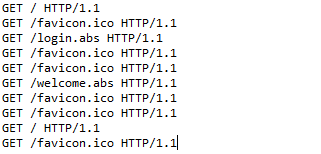
\includegraphics[
        width=0.6\textwidth
    ]{img/web-browser-request.png}
    \caption{Contoh \textit{request} dari \textit{web browser}}
    \label{fig:webBrowserRequest}
\end{figure}

\begin{figure}
    \centering
    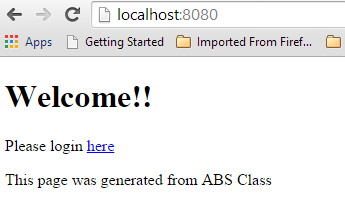
\includegraphics[
        width=0.6\textwidth
    ]{img/abs-welcome-view.png}
    \caption{Halaman web yang dibuat menggunakan ABS}
    \label{fig:javaABSCallResult}
\end{figure}

Sampai pada tahap ini penulis telah berhasil membuat sebuah halaman web sederhana dengan menggunakan ABS. Langkah berikutnya yang penulis lakukan adalah mencoba untuk memetakan ABS kedalam komponen-komponen MVC untuk membuat sebuah MVC Framework.

\section{Pemetaan ABS kedalam komponen MVC}
Salah satu tujuan dibentuknya framework MVC untuk ABS adalah agar para pengembang perangkat lunak dapat dengan mudah memisahkan kode program yang mengandung logika bisnis, data dan presentasi dari sebuah aplikasi. Oleh karena itu, sebelum membentuk sebuah framework MVC secara utuh, penulis perlu melakukan pemetaan terhadap kode ABS kedalam setiap komponen Model, View dan Controller (MVC). Tujuan dari dilakukannya proses pemetaan ini adalah agar penulis mendapatkan gambaran bagaimana seharusnya komponen Model, View dan Controller tersebut dibuat dengan menggunakan ABS.\\

Secara umum ABS memiliki sintaks yang tidak jauh berbeda dengan JAVA. Selain itu ABS juga sudah mendukung model pemrograman Object-Oriented Programming (OOP). Oleh karenanya penulis dapat menggunakan pengalaman penulis dalam menggunakan framework MVC untuk JAVA dan PHP (karena keduanya memiliki konsep OOP) beserta hasil studi literatur yang sudah penulis lakukan dalam melakukan proses pemetaan ini. Jika kita merujuk pada publikasi yang dibuat oleh \cite{krasner1988desc} dan \cite{leff2001web} tentang MVC, berikut adalah karakteristik dari masing-masing komponen MVC:

\begin{itemize}
    \item Model: merupakan bagian dari aplikasi yang merepresentasikan data pada aplikasi dan memiliki fungsi yang dapat digunakan untuk memanipulasi data sesuai dengan \textit{input} yang diberikan.
    \item View: merupakan bagian dari aplikasi yang berfungsi untuk menampilkan informasi kepada user baik dalam bentuk teks ataupun grafis.
    \item Controller: merupakan bagian dari aplikasi yang berfungsi untuk menerima, mengintepretasikan dan memproses setiap \textit{input} yang diberikan oleh \textit{user}.
\end{itemize}

Berdasarkan karakteristik di atas apabila penulis ingin membuat sebuah halaman web yang menampilkan sebuah daftar data mahasiswa (berisikan nomor mahasiswa, nama dan alamat) dalam bentuk tabel, maka komponen-komponen aplikasi yang harus penulis buat antara lain adalah (1) sebuah ABS module yang dapat merepresentasikan data mahasiswa (Model), (2) sebuah ABS module yang dapat menampilkan data mahasiswa dalam bentuk tabel (View) dam (3) sebuah ABS module yang berfungsi untuk mengintegrasikan kedua module tersebut (Controller). Berikut ini adalah module-module ABS yang penulis buat berdasarkan rincian tersebut:

\begin{lstlisting}[
caption=Module ABS untuk merepresentasikan data mahasiswa,
label={lst:absModuleMahasiswa}
]
module MMahasiswa;
export Mahasiswa, MahasiswaImpl;

interface Mahasiswa
{
	String getNpm();
	String getNama();
	String getAlamat();
}

class MahasiswaImpl(
	String npm, String nama, String alamat) implements Mahasiswa
{
	String getNpm() { return this.npm; }
	String getNama() { return this.nama; }
	String getAlamat() { return this.alamat; }
}
\end{lstlisting}

Seperti yang terlihat pada kode \ref{lst:absModuleMahasiswa} di atas, penulis membuat sebuah module ABS yang hanya berisikan atribut npm, nama dan alamat beserta method accessor-nya (\texttt{getNpm()}, \texttt{getNama()} dan \texttt{getAlamat()}). Module ini dibuat hanya mengandung atribut dan \textit{accessor} adalah karena untuk dapat merepresentasikan data Mahasiswa, module ini harus menyimpan atribut-atribut yang berhubungan dengan Mahasiswa beserta dengan \textit{method} pembantu untuk melakukan manipulasi data sesuai dengan \textit{input} yang diberikan \textit{user}.\\

Setelah berhasil membuat komponen Model \texttt{Mahasiswa}, berikutnya adalah membuat komponen View yang akan menampilkan data mahasiswa dalam bentuk tabel. Berikut adalah kode ABS yang dibuat oleh penulis dalam membuat komponen View tersebut:

\begin{lstlisting}[
caption=Module ABS untuk menampilkan data Mahasiswa dalam bentuk tabel,
label={lst:absModuleMhsView}
]
module MMahasiswaListView;
export MahasiswaListView, MahasiswaListViewImpl;
import Mahasiswa, MahasiswaImpl from MMahasiswa;

interface MahasiswaListView
{
	String generateView();
}

class MahasiswaListViewImpl
	(List<Mahasiswa> listMhs) implements MahasiswaListView
{
	String generateView()
	{
		String html = "<!DOCTYPE HTML>";
		html = html + "<html>";
		html = html + "<body>";
		html = html + "<h1>Daftar Mahasiswa</h1>";
		html = html + "<table>";
		html = html + "<thead>";
		html = html + "<tr>";
		html = html + "<td>No.</td>";
		html = html + "<td>NPM</td>";
		html = html + "<td>Nama</td>";
		html = html + "<td>Alamat</td>";
		html = html + "</tr>";
		html = html + "<tbody>";
		
		Int listLength = length(listMhs);
		Int index = 0;
		while(index < listLength)
		{
			Mahasiswa mhs = nth(listMhs, index);
			String npm = mhs.getNpm();
			String nama = mhs.getNama();
			String alamat = mhs.getAlamat();
			Int nomor = index + 1;
			
			html = html + "<tr>";
			html = html + "<td>" + toString(nomor) + "</td>";
			html = html + "<td>" + npm + "</td>";
			html = html + "<td>" + nama + "</td>";
			html = html + "<td>" + alamat + "</td>";
			html = html + "</tr>";
			index = index + 1;
		}
		
		html = html + "</tbody>";
		html = html + "</table>";
		
		return html;
	}
}
\end{lstlisting}

Kode \ref{lst:absModuleMhsView} di atas merupakan module ABS yang dibuat berdasarkan kriteria komponen View pada MVC yang sudah penulis bahas sebelumnya. Dikarenakan komponen View hanya berfungsi untuk menampilkan data yang diberikan, maka module ABS ini hanya berisi sebuah \textit{method} untuk menghasilkan sebuah halaman HTML yang akan menampilkan daftar mahasiswa.\\

Sampai tahap ini penulis sudah membuat module ABS yang merepresentasikan data Mahasiswa (kode \ref{lst:absModuleMahasiswa}), selain itu penulis juga sudah membuat sebuah module ABS yang dapat menghasilkan sebuah halaman HTML untuk menampilkan data-data mahasiswa dalam bentuk tabel (kode \ref{lst:absModuleMhsView}). Selanjutnya, penulis akan membuat satu buah module lagi yang tersisa yaitu module ABS yang bertugas untuk mengintegrasikan kedua buah module yang sudah dibuat sebelumnya. Berikut adalah kode ABS yang penulis buat untuk merealisasikan hal tersebut:

\begin{lstlisting}[
caption=Module ABS untuk mengintegrasikan antara data dan presentasi,
label={lst:absModuleMhsController},
escapeinside={@}{@}
]
module MMahasiswaController;
import MahasiswaListView, MahasiswaListViewImpl from MMahasiswaListView;
import Mahasiswa, MahasiswaImpl from MMahasiswa;

interface MahasiswaController
{
	String showMahasiswaList();
}

class MahasiswaControllerImpl 
	implements MahasiswaController
{
	String showMahasiswaList()
	{
		List<Mahasiswa> listMhs = Nil; @\label{lst:absStartCreateMhsList}@
		Mahasiswa andi = new local MahasiswaImpl(
		"1306001", "Andi", "Jl. Depok Baru");
		
		Mahasiswa budi = new local MahasiswaImpl(
		"1306002", "Budi", "Jl. Mampang Raya");
		
		Mahasiswa cita = new local MahasiswaImpl(
		"1306003", "Cita", "Jl. Irian Jaya");
		
		listMhs = appendright(listMhs, andi);
		listMhs = appendright(listMhs, budi);
		listMhs = appendright(listMhs, cita); @\label{lst:absEndCreateMhsList}@
		
		MahasiswaListView view = 
			new local MahasiswaListViewImpl(listMhs); @\label{lst:absGenerateMhsView}@
		
		String html = view.generateView(); @\label{lst:absGenerateMhsView2}@
		
		return html;
	}
}
\end{lstlisting}

Seperti yang terlihat pada kode \ref{lst:absModuleMhsController} di atas, module tersebut berperan dalam mengintegrasikan modul \texttt{Mahasiswa} dengan modul \texttt{MahasiswaListView} untuk menghasilkan sebuah halaman web yang berisi daftar mahasiswa dalam bentuk tabel. Pada kode \ref{lst:absModuleMhsController} baris \ref{lst:absStartCreateMhsList} - \ref{lst:absEndCreateMhsList} penulis membuat tiga buah objek \texttt{Mahasiswa} yang kemudian penulis masukan kedalam sebuah \texttt{List} yang merupakan representasi dari data-data Mahasiswa. Selanjutnya penulis memberikan data tersebut ke dalam objek \texttt{MahasiswaListView} untuk kemudian ditampilkan dalam bentuk HTML seperti yang tertera pada kode \ref{lst:absModuleMhsController} baris \ref{lst:absGenerateMhsView} dan \ref{lst:absGenerateMhsView2}.\\

Setelah berhasil membuat tiga buah modul yang dibutuhkan, berikutnya penulis akan memanggil modul \texttt{MahasiswaController} untuk melihat hasil dari halaman web yang dibuat. Oleh karena itu penulis menambahkan sedikit kode pada web server yang penulis buat (lihat kode \ref{lst:javaSimpleWebServer}) untuk memanggil module \texttt{MahasiswaController} tersebut. berikut adalah tambahan kode yang telah penulis buat beserta halaman web yang telah berhasil dibuat dengan menggunakan ABS.

\begin{lstlisting}[
caption=Tambahan kode pada web server untuk memanggil modul \texttt{MahasiswaController},
label={lst:javaCallMahasiswaController}
]
else if(protocols[1].equals("/listMahasiswa"))
{
    MahasiswaController_i controller = MahasiswaControllerImpl_c.__ABS_createNewObject(this);
    html = ABSRuntime.checkForNull(controller).showMahasiswaList().getString();
    out.println(html);
}
\end{lstlisting}

\begin{figure}
    \centering
    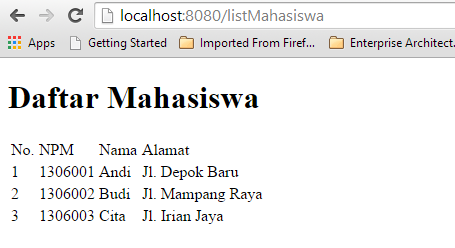
\includegraphics[
        width=0.6\textwidth
    ]{img/hasil-list-mhs.png}
    \caption{Halaman daftar mahasiswa yang dibuat menggunakan ABS}
    \label{fig:htmlDaftarMhs}
\end{figure}

Sampai pada tahap ini, penulis telah berhasil memetakan modul-modul ABS yang dibuat kedalam komponen MVC untuk menghasilkan sebuah halaman web. Namun penulis masih menemukan banyak kekurangan dalam pembuatan komponen MVC ini yang salah satu diantaranya adalah ketika kita membuat komponen view (modul \texttt{MahasiswaListView}). Jika melihat kode \ref{lst:absModuleMhsView} di atas, kode HTML yang dibuat oleh penulis masih berupa \texttt{String} yang disambung-sambung. Hal ini tentunya sangat tidak efektif terlebih lagi jika penulis ingin membuat sebuah halaman web yang lebih kompleks. Oleh karena itu, dibutuhkan adanya solusi lain untuk dapat membuat komponen view ini menjadi lebih mudah dibuat dan dikelola.

\section{Perbaikan Komponen View Menggunakan HTML Template Engine}

Berdasarkan hasil evaluasi pada percobaan sebelumnya, penulis merasa perlu untuk mengganti metode yang penulis lakukan dalam membuat komponen view dengan menggunakan ABS. Setelah dikaji lebih jauh lagi, penulis menyadari bahwa standar yang berlaku dalam membuat sebuah halaman web adalah dengan menggunakan HTML. Pada saat penulis membuat komponen view dengan menggunakan ABS untuk menghasilkan HTML, proses pembuatan komponen view menjadi lebih rumit dan kurang fleksibel. Oleh karena itu, penulis membuat keputusan untuk meninggalkan ABS dan beralih ke kode HTML murni ketika membuat komponen view aplikasi.\\

Salah satu pendekatan yang dapat dilakukan utuk mengintegrasikan ABS dengan HTML adalah dengan menggunakan HTML \textit{template engine}. Secara singkat HTML \textit{template engine} adalah sebuah perangkat lunak yang dapat digunakan para pengembang perangkat lunak untuk dapat menyematkan objek ke dalam sebuah HTML dengan menggunakan sintaks tambahan. Dengan menggunakan perangkat lunak ini, penulis dapat langsung menyematkan modul \texttt{Mahasiswa} yang telah penulis buat kedalam sebuah halaman HTML. Dalam penelitian ini, penulis menggunakan HTML \textit{template engine} berbasis JAVA yaitu Thymeleaf \footnote{http://thymeleaf.org}.

\begin{figure}
    \centering
    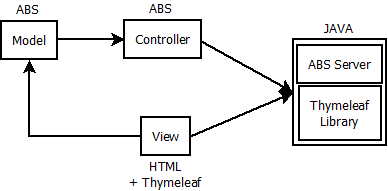
\includegraphics[
        width=0.8\textwidth]{img/alur-thymeleaf.png}
    \caption{Integrasi ABS, JAVA dan Thymeleaf}
    \label{fig:integrasiThymeleaf}
\end{figure}

Seperti yang terlihat pada gambar \ref{fig:integrasiThymeleaf}, dalam kasus ini penulis tidak langsung memanggil komponen View melalui Controller seperti yang penulis lakukan pada kode \ref{lst:absModuleMhsController}. Hal ini dilakukan karena komponen View yang dibuat dengan menggunakan thymeleaf murni menggunakan sintaks HTML sehingga tidak dapat dibuat objeknya. Penggunaan HTML dalam membuat komponen View tentunya akan mempermudah para pengembang perangkat lunak dalam membuat komponen View serta memubuat komponen view menjadi lebih rapih dan mudah dibaca. berikut perubahan pada komponen view yang penulis buat dengan menggunakan thymeleaf:

\begin{lstlisting}[
caption=Komponen View menggunakan HTML dan Thymeleaf,
label={lst:viewMhsListHTML},
escapeinside={@}{@}
]
<!DOCTYPE html>
<html>
<body>
	<h1>Daftar Mahasiswa</h1>
	<table>
		<thead>
			<tr>
				<td>No.</td>
				<td>NPM</td>
				<td>Nama</td>
				<td>Alamat</td>
			</tr>
		</thead>
		<tbody>
			<tr th:each="mahasiswa: ${mahasiswaList}"> @\label{lst:thymeStartLoop}@
				<td th:text="${#ids.seq('')}"></td>
				<td th:text="${mahasiswa.npm}"></td>
				<td th:text="${mahasiswa.nama}"></td>
				<td th:text="${mahasiswa.alamat}"></td>
			</tr> @\label{lst:thymeEndLoop}@
		</tbody>
	</table>
</body>
</html>
\end{lstlisting}

Seperti yang terlihat pada kode \ref{lst:viewMhsListHTML} di atas, penulis membuat sebuah halaman web yang equivalent dengan kode \ref{lst:absModuleMhsView} hanya saja kode ini dibuat dengan menggunakan sintaks HTML dan thymeleaf. Jika kita lihat kode \ref{lst:viewMhsListHTML} baris \ref{lst:thymeStartLoop} - \ref{lst:thymeEndLoop} terdapat sebuah sintaks yang bukan standar HTML, sintaks tersebut merupakan sintaks dari thymeleaf (bisanya dintadi dengan \texttt{th:}). Tujuan dari penggunaan sintaks tersebut adalah untuk melakukan iterasi pada sebuah \texttt{List} untuk kemudian menampilkan seluruh atribut dari objek yang berada di dalam \texttt{List} tersebut.\\

Sampai pada tahap ini penulis telah berhasil memperbaiki komponen view dari yang sebelumnya menggunakan ABS menjadi HTML dan thymeleaf sehingga membuat komponen ini menjadi lebih mudah untuk didefinisikan dan lebih sesuai dengan kebiasaan para pengembang. Akan tetapi perubahan ini belum dapat diintegrasikan secara langsung dengan komponen-komponen lainnya karena masih banyak penyesuaian yang harus dilakukan baik di tingkat \textit{web server} maupun di komponen MVC lainnya. Oleh karena itu, langkah selanjutnya yang dilakukan oleh penulis adalah mengubah \textit{web server} dan komponen MVC lainnya agar sesuai dengan implementasi komponen View yang terbaru.

\section{Integrasi Thymeleaf dengan Web Server dan ABS}

Walaupum ABS dapat dikompilasi kedalam bentuk JAVA dan Thymeleaf juga merupakan komponen perangkat lunak yang berbasis JAVA, penulis tidak dapat mengintegrasikan dua hal tersebut secara langsung di dalam Class JAVA hasi kompilasi ABS. Hal ini terjadi karena penulis tidak ingin melakukan modifikasi terhadap Class JAVA tersebut dikarenakan Class JAVA ini merupakan \textit{auto generated file} sehingga kodenya akan selalu berubah. Oleh karena itu, penulis memutuskan untuk mengintegrasikan Thymeleaf dengan komponen MVC ABS di tingkat \textit{web server}. berikut adalah langkah-langkah yang penulis ambil dalam proses integrasinya:

\begin{enumerate}
    \item Pada saat \textit{web server} menerima \textit{request} dari \textit{web browser}, \textit{web server} akan memanggil komponen Controller ABS (yang sudah dikompilasi menjadi JAVA).
    \item Komponen Controller tersebut nantinya akan memberikan data (komponen Model) dan lokasi berkas HTML yang menjadi komponen View-nya.
    \item Setelah \textit{web server} menerima data dan lokasi berkas HTML dari komponen Controller, selanjutnya \textit{web server} akan mencari berkas HTML tersebut dan membuat sebuah \texttt{Context} untuk kemudian digabungkan dengan data yang diberikan.
    \item Setelah proses penggabungan selesai dan halaman web yang diinginkan sudah terbentuk, selanjutnya \textit{web server} akan memberikan halaman web tersebut kepada web browser.
\end{enumerate}

Berikut adalah modul \texttt{MMahasiswaController} yang sudah diubah sesuai dengan rencana implementasi di atas:

\begin{lstlisting}[
caption=Module \texttt{MMahasiswaController} yang disesuaikan untuk integrasi thymeleaf,
label={lst:absMhsControllerNew},
escapeinside={@}{@}
]
module Controller.MMahasiswaController;
import Mahasiswa, MahasiswaImpl from Model.MMahasiswa;

interface MahasiswaController
{
	Pair<String, List<Mahasiswa>> showMahasiswaList(); @\label{lst:absReturnType}@
}

class MahasiswaControllerImpl implements MahasiswaController
{
	Pair<String, List<Mahasiswa>> showMahasiswaList() @\label{lst:absReturnType2}@
	{
		...
		
		return Pair("list_mahasiswa", listMhs); @\label{lst:absReturnViewAndModel}@
	}
}
\end{lstlisting}

Terlihat pada kode \ref{lst:absMhsControllerNew} baris \ref{lst:absReturnViewAndModel}, penulis tidak lagi membuat \textit{instance} dari \texttt{MahasiswaListView} melainkan hanya mengembalikan lokasi berkas HTML yang menjadi komponen View-nya berserta dengan data Mahasiswa yang akan ditampilkan kedalam halaman web. Selain itu, pada baris \ref{lst:absReturnType} dan \ref{lst:absReturnType2} juga terdapat perubahan kode yaitu dari yang sebelumya \textit{method} \texttt{showMahasiswaList} hanya mengembalikan nilai \texttt{String} berubah menjadi \texttt{Pair(String, List<Mahasiswa>)}.

Setelah melakukan perubahan pada komponen Controller, berikutnya adalah melakukan perubahan pada \textit{web server}. Berikut adalah perubahan-perubahan pada web server yang penulis lakukan untuk mengintegrasikan thymeleaf dengan ABS:

\begin{lstlisting}[
caption=Perubahan pada kode \textit{web server},
label={lst:javaNewWebServer},
escapeinside={@}{@}
]
...

else if(protocols[1].equals("/listMahasiswa")) {
   	MahasiswaController_i controller = MahasiswaControllerImpl_c.__ABS_createNewObject(this);
   	Pair<ABSString, ABS.StdLib.List<Mahasiswa_i>> pair = controller.showMahasiswaList();
   	String view = pair.getArg(0).toString().replaceAll("\"", "");
   	
   	ABS.StdLib.List<Mahasiswa_i> absData = (ABS.StdLib.List<Mahasiswa_i>) pair.getArg(1);
   	ArrayList<Object> data = new ArrayList<Object>();
           		
	do @\label{lst:javaStartConvertABSList}@
	{
		ABSObject head = (ABSObject) ABS.StdLib.head_f.apply(absData);
		data.add(head);
		
		absData = ABS.StdLib.tail_f.apply(absData);
	}
	while(!(absData instanceof ABS.StdLib.List_Nil)); @\label{lst:javaEndConvertABSList}@
	
	TemplateResolver templateResolver = new TemplateResolver(); @\label{lst:javaStartThymeleaf}@
    templateResolver.setTemplateMode("XHTML");
    templateResolver.setSuffix(".html");
    templateResolver.setResourceResolver(new ResourceResolver()); @\label{lst:javaCallResourceResolver}@
                
    TemplateEngine templateEngine = new TemplateEngine();
    templateEngine.setTemplateResolver(templateResolver);
                
	Context ctx = new Context(); @\label{lst:javaCreateContext}@
	StringWriter writer = new StringWriter();
	ctx.setVariable("mahasiswaList", data); @\label{lst:javaThymeSetData}@
	templateEngine.process(view, ctx, writer); @\label{lst:javaThymeProcess}@
	
	out.println(writer); @\label{lst:javaEndThymeleaf}@
}

...
\end{lstlisting}

Jika kita membandingkan kode \ref{lst:javaNewWebServer} di atas dengan kode \ref{lst:javaCallMahasiswaController} yang telah dibuat sebelumnya, terdapat banyak perubahan pada cara web server membuat sebuah halaman web. Pada kode \ref{lst:javaCallMahasiswaController} \textit{web server} langsung mendapatkan halaman web pada saat melakukan pemanggilan \texttt{MahasiswaController} Sedangkan pada kode \ref{lst:javaNewWebServer} proses pembuatan halaman web dilakukan \textit{web server}. Seperti yang terlihat pada kode \ref{lst:javaNewWebServer} baris \ref{lst:javaStartConvertABSList} sampai \ref{lst:javaEndConvertABSList}, \textit{web server} melakukan proses konversi data dari \texttt{ABSList} menjadi \texttt{List}. Hal ini dilakukan karena Thymeleaf hanya mengenali \textit{JAVA Collection} bawaan dari JAVA API sedangkan \texttt{ABSList} bukan merupakan bawaan dari JAVA API.\\

Setelah \textit{web server} selesai melakukan konversi data, berikutnya adalah memasukan data tersebut ke dalam komponen View yang sudah dibuat. Proses ini dilakukan dengan cara me-\textit{load} berkas HTML yang dilakukan oleh sebuah Class khusus yang bernama \texttt{ResourceResolver} (lihat kode \ref{lst:javaResourceResolver}) dan menggabungkan berkas tersebut dengan data yang ada kedalam sebuah \texttt{Context} untuk kemudian diproses menjadi sebuah halaman web (lihat kode \ref{lst:javaNewWebServer} baris \ref{lst:javaCreateContext} sampai \ref{lst:javaThymeProcess}).

\begin{lstlisting}[
caption=Class \texttt{ResourceResolver} sebagai tambahan pada \textit{web server},
label={lst:javaResourceResolver}
]
public class ResourceResolver implements IResourceResolver
{
	...
	
	public InputStream getResourceAsStream(TemplateProcessingParameters templateProcessingParameter,
			String resourceName) 
	{
		
		Validate.notNull(resourceName, "Resource name cannot be null");
		return ResourceResolver.class.getResourceAsStream("/" + resourceName);
	}

}
\end{lstlisting}

\begin{figure}
    \centering
    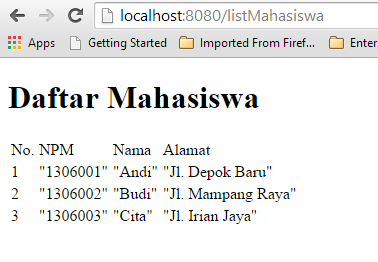
\includegraphics[width=0.6\textwidth]{img/hasil-list-mhs_new.png}
    \caption{Halaman Web yang dihasilkan oleh ABS dan Thymeleaf}
    \label{fig:listMhsThymeleaf}
\end{figure}

Sampai pada tahap ini, penulis telah berhasil mengintegrasikan komponen View yang menggunakan HTML dengan komponen Controller dan Model yang dibuat dengan menggunakan ABS (lihat hasilnya pada gambar \ref{fig:listMhsThymeleaf} di atas). langkah selanjutnya adalah menggabungkan seluruh hasil eksperimen yang sudah dilakukan menjadi sebuah \textit{framework} MVC ABS.